%! Author = sari3
%! Date = 10.06.2024

% Preamble
\documentclass[12pt]{article}


\usepackage[utf8]{inputenc} % Eingabekodierung
\usepackage[T1]{fontenc} % Ausgabe-Kodierung
\usepackage[ngerman]{babel} % Deutsche Spracheinstellungen

% Packages
\usepackage{amsmath}
\usepackage{listings}
\usepackage{xcolor}
\usepackage{graphicx}



\lstset{
    language=Python, % Beispielhaft: Programmiersprache
    breaklines=true, % Zeilenumbruch aktivieren
    breakatwhitespace=true, % Zeilenumbruch an Leerzeichen
    basicstyle=\ttfamily\small, % Schriftart und -größe für den Code
    keywordstyle=\color{blue}, % Farbe für Schlüsselwörter
    stringstyle=\color{red}, % Farbe für Strings
    commentstyle=\color{gray}, % Farbe für Kommentare
    frame=single, % Rahmen um den Code
    columns=flexible, % Korrekte Handhabung der Zeichenbreite
    keepspaces=true, % Behandelt Leerzeichen korrekt
    xleftmargin=2em, % Linker Rand für den Codeblock
    xrightmargin=2em, % Rechter Rand für den Codeblock
    showspaces=false, % Leerzeichen nicht anzeigen
    showstringspaces=false % Leerzeichen in Strings nicht anzeigen
}




\title{% \vfill
%\vspace{-2.0cm}
    3D-Puzzle mit Greifarm}
\author{
    Maja Wantke \texttt{mwantke@stud.hs-bremen.de} \and
    Lara Miritz \texttt{lmiritz@stud.hs-bremen.de} \and
    Nikias Scharnke \texttt{nscharnke@stud.hs-bremen.de} \and
    Sara-Ann Wong \texttt{swong@stud.hs-bremen.de} \\
    Angewandte Mathematik für Medieninformatik \\
    Hochschule Bremen}
\date{ \today}
\parindent 0pt
\parskip 1ex

% Document
\begin{document}

    \maketitle

    \begin{abstract}
        Diese Dokumentation beschreibt die Entwicklung und Implementierung einer 2D Roboterarm Simulation,
        die Konzepte der Kinematik praxisnah veranschaulicht. Die Simulation ermöglicht es, einen Roboterarm
        interaktiv zu steuern und Puzzleteile zu bewegen. Nutzer können den Roboterarm selbst konfigurieren
        und so die Komplexität der Steuerung kennenlernen.
    \end{abstract}
    \clearpage
    \tableofcontents
    \clearpage
    \listoffigures
    \clearpage


    \section{Motivation}
    Roboterarmsimulationen sind ein wesentlicher Bestandteil der Robotikforschung. Sie ermöglichen es,
    komplexe Bewegungsabläufe zu visualisieren und zu verstehen. Unser Projekt soll eine benutzerfreundliche
    und interaktive Anwendung bereitstellen, die es dem Benutzer ermöglicht, die Funktionsweise eines
    Roboterarms durch direkte Interaktion zu erforschen. Der Benutzer kann dabei selbst experimentieren
    und forschen, um eigene Erkenntnisse über die Bewegungssteuerung und Kinematik des Roboterarms zu gewinnen.
    Dies fördert das Verständnis und die Fähigkeit, theoretisches Wissen in die Praxis umzusetzen.


    \section{Verwandte Arbeiten}
    Unser Projekt wurde durch verschiedene Arbeiten im Bereich der Roboterarmsimulation inspiriert.
    Die Bachelorarbeit zur „Steuerung eines 5-DOF Handhabungsroboters in Arbeitsraumkoordinaten“[1] von Julia
    Dubcova erklärt die Grundlagen der Robotersteuerung und der inversen Kinematik, die wir für unseren
    Roboterarm nutzen. Eine weitere wichtige Quelle war die Veröffentlichung „Tactile Robotic Assembly“[2]
    vom BBSR. Diese half uns, die Interaktion des Roboterarms mit Objekten zu verstehen. Beide Arbeiten haben
    uns wertvolle Ideen und Techniken geliefert, die wir in unserer interaktiven Roboterarmsimulation anwenden
    wollen. Ergänzend haben wir uns auch an der Arbeit „Robot Arm Control using Machine Learning“[3] orientiert,
    welche moderne Ansätze zur Steuerung von Roboterarmen mittels maschinellem Lernen beleuchtet. Zur Umsetzung
    der Animationen orientieren wir uns an der neuesten Auflage des Werkes „Computer Animation: Algorithms and
    Techniques“[4] von Rick Parent, die unter anderem die Grundlagen der Animationsprogrammierung vermittelt.
    Es behandelt Grundlagen wie Bewegung, Deformation und physikalische Simulation, um realistische Animationen
    zu erstellen.


    \section{Projektübersicht}
    In diesem Projekt wurde ein 2D-Puzzle-Spiel entwickelt, das durch einen Roboter-Greifarm gelöst werden
    muss. Der Greifarm wird durch Drag & Drop interaktiv gesteuert und verwendet inverse Kinematik, um
    Bewegungen präzise auszuführen. Diese Steuerung ermöglicht es dem Benutzer, die Komplexität der
    Roboterbewegungen zu verstehen und verschiedene Konfigurationen des Arms auszuprobieren.

    Der Benutzer kann Ziele per Mausinteraktion festlegen, die der Roboterarm erreichen soll, und Puzzleteile
    greifen, um sie an eine Position im Raster zu verschieben. Dabei wird eine Kollisionserkennung verwendet,
    die überprüft, ob eine Kollision zwischen einem Puzzleteil und dem Raster auftritt. Ist dies der Fall, so
    rastet das Puzzleteil im Raster ein. Durch diese interaktive und benutzerfreundliche Anwendung erhält der
    Benutzer die Möglichkeit, die Funktionsweise eines Roboterarms praktisch zu erforschen und dabei eigene
    Experimente durchzuführen. Dies fördert ein tieferes Verständnis der Bewegungsabläufe und der Kinematik
    von Roboterarmen und ermöglicht wertvolle Erkenntnisse durch direkte Interaktion.


    \section{Entwicklungsprozess}
    Der Entwicklungsprozess begann mit der Ideenfindung und Planung, bei der verschiedene Konzepte für die
    Entwicklung eines Spiels, das von einem Roboterarm gelöst werden sollte, erörtert wurden. Das Ziel war es,
    eine benutzerfreundliche Anwendung zu schaffen, die es Nutzern ermöglicht, die Funktionsweise eines
    Roboterarms durch direkte Interaktion zu erforschen.

    Am 10. Juni 2024 wurde das Exposé abgegeben. Zu diesem Zeitpunkt wurde eine Grundstruktur der Anwendung
    erstellt, die das Layout und die grundlegenden Funktionen umfasste. Diese Struktur bildete die Grundlage
    für die weitere Entwicklung.

    Die erste Besprechung, die am 26. Juni 2024 stattfand, ermöglichte eine umfassende Überprüfung des
    bisherigen Fortschritts. Dabei wurde entschieden, die Konfiguration der Anwendung zu erweitern, um den
    Nutzern eine detailliertere Untersuchung der Kinematik des Roboterarms zu ermöglichen. Diese Erweiterung
    war nicht von Anfang an geplant, sondern entstand aus der Erkenntnis heraus, den Benutzern mehr
    Flexibilität bei der Erkundung der Armkinematik zu bieten.

    Am 12. Juli 2024 wurde der aktuelle Stand der Entwicklung vorgestellt. In dieser Präsentation lag der
    Schwerpunkt auf der neuen Konfiguration, die es den Nutzern ermöglicht, die Kinematik des Roboterarms
    selbst zu erforschen. Die Demonstration zeigte, wie Benutzer verschiedene Parameter anpassen und die
    Auswirkungen dieser Anpassungen in Echtzeit beobachten konnten. Diese Funktion ermöglichte eine tiefere
    Interaktion mit der Anwendung und stellte einen wesentlichen Fortschritt im Vergleich zur ursprünglichen
    Planung dar.

    Vor der Präsentation wurden umfassende Tests durchgeführt, um die Funktionsfähigkeit der Implementierung
    sicherzustellen. Dazu gehörten Unittests zur Überprüfung der verschiedenen Komponenten der Anwendung,
    einschließlich der Kollisionserkennung und der Drag-and-Drop-Funktionalität. Diese Tests stellten sicher,
    dass alle Funktionen stabil und fehlerfrei arbeiteten.

    Nach der Präsentation am 12. Juli 2024 wurde noch eine neue Variante, den Roboterarm mit 3 Gelenken zu
    steuern, hinzugefügt, sodass die Maus mit dem Endeffektor überlappt und man die volle Kontrolle bei der
    Steuerung hat. Daneben lag der Fokus auf der Dokumentation und dem Abschlussbericht, in dem die
    Implementierung, die Ergebnisse und das Feedback aus der Präsentation zusammengefasst wurden. Die
    abschließende Bewertung reflektierte die erfolgreiche Umsetzung des Projekts und bot Raum für mögliche
    Verbesserungsvorschläge für zukünftige Entwicklungen.


    \section{Erweiterungsmöglichkeiten}
    Das Projekt bietet mehrere Ansatzpunkte für zukünftige Erweiterungen. Eine wesentliche Möglichkeit besteht
    in der Erweiterung der Konfigurationsmöglichkeiten des Roboterarms. Derzeit können Benutzer grundlegende
    Parameter anpassen, um die Kinematik des Arms zu erforschen. Zukünftige Entwicklungen könnten es ermöglichen,
    noch detailliertere Aspekte der Armkonfiguration zu verändern. Dazu könnten erweiterte Optionen zur
    Feinabstimmung der Gelenkwinkel und Geschwindigkeiten gehören sowie zusätzliche Konfigurationsparameter,
    die eine noch präzisere Anpassung und Untersuchung der Bewegungsabläufe ermöglichen.

    Neben den funktionalen Erweiterungen besteht auch die Möglichkeit zur Verbesserung des Designs der
    Benutzeroberfläche. Die aktuelle Benutzeroberfläche bietet eine funktionale Grundstruktur, jedoch besteht
    Potenzial für eine ansprechendere und intuitivere Gestaltung. Eine Überarbeitung könnte visuelle Hilfsmittel,
    wie interaktive Anleitungen und ansprechende Grafiken, beinhalten. Solche Verbesserungen könnten die
    Benutzerfreundlichkeit erhöhen und die Lernkurve für neue Benutzer verringern, indem sie eine klarere
    und intuitivere Navigation durch die Simulation ermöglichen.


    \section{Schlussfolgerung}
    Das entwickelte 2D-Puzzle-Spiel mit Roboterarmsteuerung bietet eine solide Grundlage für die interaktive
    Simulation von Roboterkinematik. Durch die Möglichkeit, verschiedene Konfigurationen des Roboterarms zu
    testen, können Benutzer ein tieferes Verständnis für die Funktionsweise und Bewegungsabläufe von Roboterarmen
    entwickeln. Die flexible Konfigurationsmöglichkeit und die Drag-and-Drop-Funktionalität haben sich als
    zentrale Merkmale der Anwendung herausgestellt.

    Während der Umsetzung des Projekts haben wir wertvolle Erkenntnisse gewonnen. Besonders hervorzuheben
    ist, dass die Implementierung eines Roboterarms mit drei Gelenken deutlich komplexer und fehleranfälliger
    war als ursprünglich erwartet. Die Herausforderungen bei der mathematischen Modellierung und der
    kinematischen Steuerung haben gezeigt, wie anspruchsvoll die Entwicklung eines solchen Systems sein kann.
    Bei der Simulation traten immer wieder Schwierigkeiten auf, insbesondere bei der exakten Positionierung der
    Endeffektoren. Die präzise Berechnung der Gelenkwinkel und deren Koordination erwiesen sich als komplexe
    Aufgaben, die häufig Anpassungen und Fehlersuche erforderten. Erst durch eine neue Herangehensweise gelang
    die genaue Positionierung der Endeffektors. Trotz der sorgfältigen Planung und Implementierung sind weiterhin
    Verbesserungen und Erweiterungen möglich, um die Funktionalität und Benutzerfreundlichkeit weiter zu
    optimieren. Die gesammelten Erfahrungen haben unsere Kenntnisse in der Roboterkinematik und der praktischen
    Anwendung von Simulationstechniken erheblich erweitert.


    \section{Implementierung}

    \subsection{Gegenstand der Entwicklung}
    In einer zweidimensionalen Umgebung soll ein Puzzlespiel entstehen, das mit Hilfe eines Roboterarms
    gesteuert wird. Dieser Arm kann per Drag-and-Drop gesteuert werden und so die einzelnen Puzzleteile
    erreichen und aufheben. Die Anzahl der Gelenke und die Länge der einzelnen Armteile sind dabei über
    ein Menü variabel einstellbar. Sobald das Puzzle gelöst ist, kann es mit Hilfe einer Korrekturfunktion
    überprüft werden.

    \subsection{Roboterarm}
    Um den Roboterarm später steuern zu können, muss dieser zunächst in einer eigenen Klasse konfiguriert
    werden. Dabei wird er mit Startwerten versehen und erhält Methoden, die die Positionen des Roboterarms
    bei der Bewegung neu berechnen.

    \subsubsection{Initialisierung}
    Um später beim Starten des Programms einen Roboterarm sehen zu können, muss dieser initialisiert
    werden. Dabei werden die Anzahl der Gelenke auf zwei sowie die Winkel der drei möglichen Gelenke
    auf 0 Grad festgelegt. Die Länge der einzelnen Armteile wurde zuvor als Konstante festgelegt auf
    jeweils 150 eingestellt.

    \lstinputlisting[language=Python, firstline=15, lastline=44]{PuzzleSpiel.py}

    \subsubsection{Berechnung Winkel}
    Während der Arm bewegt wird, werden dauerhaft die Winkel in den Gelenken neu berechnet, um den
    Endeffektor erreichen zu können. Benötigt werden dafür die Differenzen der x- und y-Koordinaten
    zwischen dem Endeffektor und dem Schultergelenk beziehungsweise dem Ursprung. Mit diesen kann durch
    den Satz des Pythagoras die Distanz bestimmt werden, die zur Berechnung der Winkel notwendig ist.

    \[
        c = \sqrt{a^2 + b^2}
    \]
    \[
        c = \sqrt{80^2 + 60^2} = 100
    \]

    \begin{figure}[h!]
        \centering
        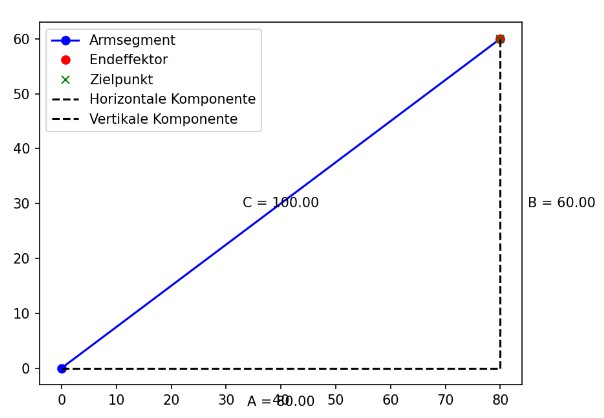
\includegraphics[width = \linewidth]{Bild 1}
        \caption{Berechnung Distanz}
    \end{figure}


    \lstinputlisting[language=Python, firstline=56, lastline=60]{PuzzleSpiel.py}


    Für die Berechnung bei 1, 2 und 3 Gelenken ist unterschiedlicher Code erforderlich. Dieser wird je
    nach Bedarf durch eine if-else-Anweisung aufgerufen.

    \subsubsubsection{Berechnung für 1 Gelenk}
    Handelt es sich um nur ein Gelenk, soll der Endeffektor des Arms in Richtung des Zielpunkts
    bewegt werden. Für die genauen Koordinaten wird die zuvor berechnete Distanz und der Winkel des
    Armsegments benötigt. Diesen erhält man durch Einsetzen der Koordinaten in die
    Arcustangens-Funktion.

    \[
        \theta=arctan(\frac{B}{A})
    \]
    \[
        \theta=arctan(\frac{60}{80})=0,64 (36,87^\circ)
    \]

    \begin{figure}[h]
        \centering
        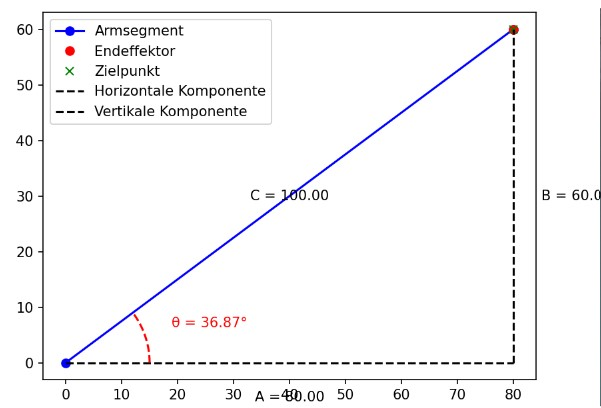
\includegraphics[width = \linewidth]{Bild 2}
        \caption{Berechnung Schulterwinkel für 1 Armsegment}
    \end{figure}

    \lstinputlisting[language=Python, firstline=62, lastline=69]{PuzzleSpiel.py}

    Multipliziert man nun die Armlänge mit dem Sinus beziehungsweise dem Kosinus des Winkels, erhält
    man den Endeffektor.

    \[
        x=c * cos(\theta)
    \]
    \[
        y=c * sin(\theta)
    \]
    \[
        x=100 * cos(0,64)=80
    \]
    \[
        y=100 * sin(0,64)=60
    \]

    \lstinputlisting[language=Python, firstline=136, lastline=140]{PuzzleSpiel.py}


    \subsubsubsection{Berechnung für 2 Gelenke}
    Bei der Berechnung der Winkel mit zwei Armsegmenten wird wie bei einem Armsegment auch zuerst
    die Distanz zwischen dem Endeffektor und dem Ursprung berechnet. Zusätzlich sind die Längen der
    beiden Armsegmente gegeben, woraus ein Dreieck mit drei bekannten Seitenlängen entsteht.

    \begin{figure}[h]
        \centering
        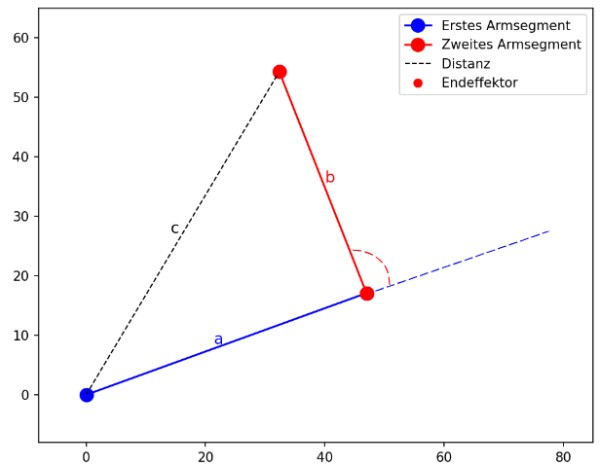
\includegraphics[width = \linewidth]{Bild 3}
        \caption{Berechnung Ellenbogenwinkel für 2 Armsegmente}
    \end{figure}

    \[
        a=50
    \]
    \[
        b=40
    \]
    \[
        c=63,25
    \]

    Für die Berechnung des Ellenbogenwinkels kann nun der Kosinussatz umgestellt nach dem Winkel
    angewendet werden.

    \[
        cos(\theta)= \frac{a^2+b^2-c^2}{2*a*b}
    \]
    \[
        cos(\theta)= \frac{50^2+40^2-63,25^2}{2*20*40}
    \]
    \[
        \theta= arccos(0,025) = 89,86^\circ
    \]

    Nachdem der Ellenbogenwinkel berechnet wurde, kann mit dessen Hilfe auch der Schulterwinkel
    berechnet werden, indem folgende Formel verwendet wird.

    \[
        \alpha = arctan(\frac{y}{x}) - arctan(\frac{b*cos(\theta)}{a+b*sin(\theta)})
    \]
    \[
        \alpha = arctan(\frac{20}{60}) - arctan(\frac{40*cos(89,86^\circ)}{50+40*sin(89,86^\circ)})                    \]
    \[
        \alpha = 18,43^\circ - 37,97^\circ = -19,55^\circ
    \]

    \lstinputlisting[language=Python, firstline=72, lastline=85]{PuzzleSpiel.py}

    Nachdem beide Winkel berechnet wurden, kann mit Hilfe der Armlängen der Arm konstruiert werden.
    Die Positionen des Ellenbogengelenks und des Endeffektors werden durch Einsetzen der Winkel in
    Sinus- und Kosinusfunktionen multipliziert mit der Armlänge bestimmt.

    Ellenbogengelenk:

    \[
        x1 = a * cos(\theta)
    \]
    \[
        y1 = a * sin(\theta)
    \]

    \[
        x1 = 50 * cos(-19,55^\circ) = 47,12
    \]
    \[
        y1 = 50 * sin(.19,55^\circ) = 16,73
    \]

    Endeffektor:

    \[
        x2 = x1 + b * cos(\theta + \alpha)
    \]
    \[
        y2 = y1 + b * sin(\theta + \alpha)
    \]

    \[
        x2 = 47,12 + 40 * cos(-19,55^\circ + 89,86^\circ) = 60,6
    \]
    \[
        y2 = 16,73 + 40 * sin(-19,55^\circ + 89,86^\circ) = 54,4
    \]

    Diese Punkte werden miteinander verbunden und werden dauerhaft aktualisiert, wodurch der
    Roboterarm dargestellt wird und sich den Bewegungen anpasst.

    \lstinputlisting[language=Python, firstline=141, lastline=145]{PuzzleSpiel.py}

    \subsubsubsection{Berechnung für 3 Gelenke}
    Die Winkel für die 3 Gelenke können auf verschiedene Weisen berechnet werden. Für die erste
    Implementierung wurden wie zuvor nur Formeln der Trigonometrie verwendet. Dort wird der
    Roboterarm von der Ellbogen-Position aus gesteuert. Hier hat man sich zunutze gemacht, dass
    der Ellbogen- und Handgelenk-Winkel derselbe aber gespiegelt sein kann.
    Erstmal muss sichergegangen werden, dass das Ziel in Reichweite liegt:

    \[
        \sqrt{100^2 + 20^2} < 60 + 50 +70
    \]
    \[
        102 < 180
    \]

    \lstinputlisting[language=Python, firstline=91, lastline=94]{PuzzleSpiel.py}

    \begin{figure}[h]
        \centering
        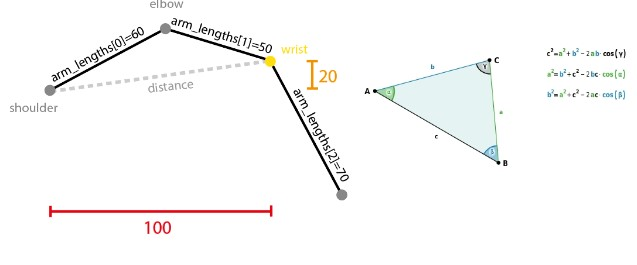
\includegraphics[width = \linewidth]{Bild 4}
        \caption{Kosinussatz}
    \end{figure}

    Kosinussatz:
    \[
        elbowangle = arccos(\frac{(100^2 +20^2)-60^2-50^2}{2*60*50}) = 0,77
    \]

    \lstinputlisting[language=Python, firstline=97, lastline=99]{PuzzleSpiel.py}

    \[
        k1 = 60 +50 * cos(0,77) = 96
    \]
    \[
        k2 = 50*sin(0,77) = 35
    \]
    \[
        shoulderangle = arctan(\frac{20}{100}) - arctan(\frac{35}{96}) = -0,15
    \]

    \lstinputlisting[language=Python, firstline=101, lastline=103]{PuzzleSpiel.py}

    \[
        wristtarget = [100, 20] - [70 * cos(0,77 - 0,15), 70* sin(0,77 -0,15)] = [43, -21]
    \]

    \[
        wristdx = 43 - 200 = -157
    \]

    \[
        wristdx = -21 - 200 = -221
    \]

    \[
        wristangle1 = arctan(\frac{-221}{.157})= 0,95
    \]
    \[
        writsangle = 0,77 -0,15 -0,95 = -0,33
    \]

    \lstinputlisting[language=Python, firstline=106, lastline=109]{PuzzleSpiel.py}

    Eine zweite Implementierung nutzt die Formeln, die man durch die gegebenen Werte aufstellen kann, um die fehlenden
    Winkel rauszubekommen. Das geschieht durch ein numerisches Optimierungsverfahren, das darauf abzielt, die Differenzen
    zwischen den berechneten Werten und den zuvor gegebenen Winkeln zu minimieren.
    Die beiden Formeln werden aus der folgenden Skizze ersichtlich:

    \begin{figure}[h]
        \centering
        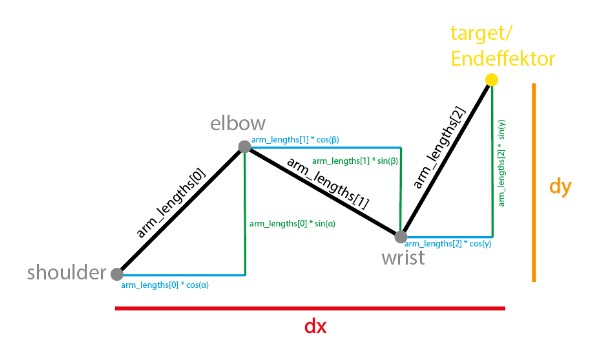
\includegraphics[width = \linewidth]{Bild 5}
        \caption{Bestimmung Endeffektor für 3 Armsegmente}
    \end{figure}

    \[
        dx = armlengths[0] * cos(\alpha) + armlengths[1] * cos(\beta) + armlength[2] * cos(\gamma)
    \]
    \[
        dx = armlengths[0] * sin(\alpha) + armlengths[1] * sin(\beta) + armlength[2] * sin(\gamma)
    \]

    \lstinputlisting[language=Python, firstline=124, lastline=133]{PuzzleSpiel.py}

    \begin{figure}[h]
        \centering
        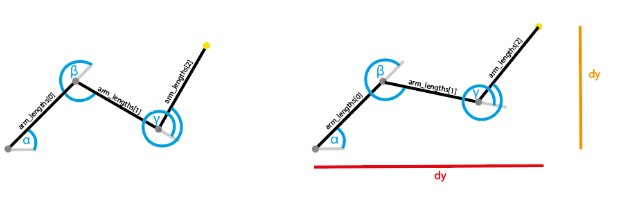
\includegraphics[width = \linewidth]{Bild 6}
        \caption{Winkelberechnung bei 3 Armsegmenten}
    \end{figure}

    In dem Beispiel ist die Ausgangsposition vom Roboterarm auf der linken Skizze abgebildet und die
    Winkel und Armlängen sind:

    \[
        \alpha = 0,5*\pi
    \]
    \[
        \beta = 1,5 * \pi
    \]
    \[
        \gamma = 2,5 * \pi
    \]

    \[
        armlengths[0] = 100
    \]
    \[
        armlengths[1] = 105
    \]
    \[
        armlengths[2] = 110
    \]

    \[
        dx = 250
    \]
    \[
        dy = 150
    \]

    Diese Werte werden zum Initial Guess, das sind die Winkel, an denen sich der Algorithmus
    orientiert.

    \lstinputlisting[language=Python, firstline=114, lastline=114]{PuzzleSpiel.py}

    Die Formeln sähen mit den gegebenen Werten folgendermaßen aus:

    \[
        0 = 100 * cos(\alpha) + 105 * cos(\beta) + 110 * cos(\gamma) -250
    \]
    \[
        0 = 100 * sin(\alpha) + 105 * sin(\beta) + 110 * sin(\gamma) -150
    \]

    Nun wird mit den obigen aufgestellten Formeln und den Orientierungswerten der least squares-
    Algorithmus aufgerufen. In dem Ergebnis sind dann die optimalen Winkel für den Roboterarm.

    \lstinputlisting[language=Python, firstline=116, lastline=118]{PuzzleSpiel.py}

    Das Ergebnis der Rechnung lautet somit:
    \[
        self.shoulderangle = 0,27 *\pi
    \]
    \[
        self.elbowangle = 1,72 *\pi
    \]
    \[
        self.wristangle = 2,25 *\pi
    \]

    Schließlich müssen auch noch die Positionen aller Gelenke und des Endeffektors berechnet werden.
    Das Verfahren unterscheidet sich gar nicht, zudem wie man in der ersten Variante vorgehen würde.
    Die Position der Schulter, welche sich beim Bewegen des Roboterarmes nicht mitbewegt, liegt bei
    [200, 200].

    \[
        elbow = [200, 200] + [100 * cos(0,27 * \pi), 100 * sin(0,27*\pi)] = [266, 275]
    \]
    \[
        wrist = [266, 275] + [105 * cos(0,27 * \pi + 1,72 * \pi), 105 * sin(0,27*\pi + 1,72 * \pi)] = [371, 272]
    \]
    \[
        endeffector = [371, 272] + [ 110 * cos(0,27*\pi + 1,72*\pi + 2,25*\pi), 110 * sin(0,27*\pi + 1,72*\pi + 2,25*\pi)] = [451, 347]
    \]

    \lstinputlisting[language=Python, firstline=146, lastline=152]{PuzzleSpiel.py}

    \subsection{GUI-Klasse}
    Die GUI-Klasse initialisiert die Hauptkomponenten der Benutzeroberfläche. Sie erstellt ein Canvas-Widget,
    auf dem der Roboterarm und die Puzzleteile angezeigt werden, sowie verschiedene Konfigurationsoptionen für
    die Steuerung des Roboterarms.

    \subsubsection{Konfigurationspanel}
    Das Konfigurationspanel ermöglicht es dem Benutzer, die Anzahl der Gelenke sowie die Längen der Arme
    des Roboterarms anzupassen. Diese Einstellungen werden dabei dynamisch aktualisiert, sodass Änderungen
    in Echtzeit umgesetzt und visuell dargestellt werden.

    \lstinputlisting[language=Python, firstline=187, lastline=238]{PuzzleSpiel.py}

    Die Methoden “update\_num\_joints()”, “update\_arm\_length1()”,
    ”update\_arm\_length2()” und
    “update\_arm\_length3()” dienen dazu, die Parameter des Roboterarms zu aktualisieren und ihn
    anschließend neu zu zeichnen.
    Die Methode “update\_num\_joints()” aktualisiert die Anpassungsmöglichkeiten des Roboterarms. Je nach
    der gewählten Anzahl der Gelenke werden die entsprechenden Konfigurationsoptionen des Roboterarms
    angezeigt oder ausgeblendet. Nach der Aktualisierung wird der Roboterarm neu gezeichnet, um die
    Änderungen visuell darzustellen.

    \lstinputlisting[language=Python, firstline=236, lastline=248]{PuzzleSpiel.py}

    \subsubsection{Puzzleteile und Grid (Zielfläche)}
    Die Puzzleteile werden erstellt und zufällig auf dem Canvas platziert. Ein 2x2-Grid dient als
    Zielbereich für die Puzzleteile. Ein Bild ist hinterlegt, aus welchem die Puzzleteile erstellt werden.
    Vorerst bildet ein 2x2-Grid bestehend aus Quadraten das Zielfeld, in welches die Puzzleteile
    hineingelegt werden sollen. Auf dieser Basis wird das Bild auf die benötigte Größe skaliert, sodass
    das Zielfeld vom Bild abgedeckt wird. Anschließend werden die Puzzleteile mit der vorher definierten
    Feldgröße erstellt, indem entsprechend große Teile aus dem Bild ausgeschnitten werden. Jedes
    Puzzleteil wird mit einem Eventlistener verbunden und in eine Liste von Puzzleteilen hinzugefügt.

    \lstinputlisting[language=Python, firstline=250, lastline=267]{PuzzleSpiel.py}


    Das Grid wird auf ähnliche Weise erstellt wie die Puzzleteile. Hierbei werden Quadrate in der zuvor
    definierten Feldgröße ohne Lücken aneinandergesetzt. Abschließend wird jedem Quadrat eine Position
    zugewiesen.

    \lstinputlisting[language=Python, firstline=269, lastline=279]{PuzzleSpiel.py}

    \subsubsection{Puzzleteile bewegen}
    Um den Roboterarm zu bewegen, muss dieser mit einem Linksklick ausgewählt werden. Dabei wird zunächst
    überprüft, ob sich der Abstand zwischen dem Mauszeiger und dem Endeffektor innerhalb eines Radius
    von 10 befindet.

    \lstinputlisting[language=Python, firstline=288, lastline=291]{PuzzleSpiel.py}
    \lstinputlisting[language=Python, firstline=328, lastline=331]{PuzzleSpiel.py}

    Während der Bewegung des Arms wird die Methode “on\_drag()” kontinuierlich ausgeführt. In diesem
    Prozess werden fortlaufend die Position des Endeffektors sowie die des ausgewählten Puzzleteils an
    die Position des Mauszeigers angepasst.

    \lstinputlisting[language=Python, firstline=293, lastline=302]{PuzzleSpiel.py}

    \subsubsection{Puzzleteile aufnehmen und ablegen}
    Durch einen Rechtsklick soll der Endeffektor ein Puzzleteil „greifen“ können. Falls der Greifarm noch
    kein Puzzleteil aufgenommen hat, wird ihm das Puzzleteil zugewiesen, dessen Koordinaten mit der
    Position des Endeffektors übereinstimmen. Danach wird der Endeffektor zentriert auf das Puzzleteil
    positioniert.

    Wenn der Greifarm bereits ein Puzzleteil aufgenommen hat, werden die Koordinaten des Puzzleteils mit
    den Koordinaten der Quadrate im Zielfeld verglichen. Ein Puzzleteil wird auf einem Quadrat platziert,
    wenn der Abstand zwischen den Koordinaten kleiner als 3 ist. Diese Bedingung wird durch den logischen
    Ausdruck in der Methode “is\_inside()” überprüft. Ist dies zutreffend, wird das Puzzleteil auf das
    entsprechende Quadrat im Grid gesetzt. Diese Vorgehensweise trägt zur Verbesserung der
    Benutzerfreundlichkeit bei.

    \lstinputlisting[language=Python, firstline=308, lastline=326]{PuzzleSpiel.py}
    \lstinputlisting[language=Python, firstline=379, lastline=389]{PuzzleSpiel.py}

    \subsubsection{Überprüfung der Position}
    Die Überprüfung beginnt erst nach Betätigung des Knopfes „Check Positions“. Bei diesem Schritt
    werden die hinterlegten Positionen der Puzzleteile mit den aktuellen Positionen verglichen, um
    sicherzustellen, dass alle Teile korrekt platziert sind. Ein Zähler wird nur dann erhöht, wenn die
    Positionen der Puzzleteile mit den vorgegebenen Positionen übereinstimmen. Dieser Zähler gibt nach
    der Überprüfung an, wie viele Puzzleteile korrekt positioniert wurden.

    \lstinputlisting[language=Python, firstline=364, lastline=377]{PuzzleSpiel.py}

    \subsection{Kollisionserkennung}
    Diese Mechanismen tragen dazu bei, eine präzise und benutzerfreundliche Interaktion mit dem
    Roboterarm und den Puzzleteilen zu gewährleisten. Die Kollisionserkennung ist entscheidend für
    die korrekte Funktionalität der Anwendung und die Genauigkeit der Interaktionen.

    \subsubsection{Kollisionserkennung beim Drag \& Drop von Puzzleteilen}
    Ein zentraler Aspekt der Kollisionserkennung betrifft das Drag & Drop von Puzzleteilen. Hierbei wird
    die Methode “on\_right\_click(self, event)” verwendet, um den Greifarm Puzzleteile mit der rechten
    Maustaste aufnehmen oder ablegen zu lassen. Um sicherzustellen, dass das Puzzleteil korrekt auf
    einem Quadrat positioniert wird, wird die Methode “is\_inside(self, square\_coords, piece\_coords)”
    verwendet. Diese Methode überprüft, ob die Randkoordinaten des Puzzleteils innerhalb der Grenzen
    eines Grid-Quadrats liegen, wobei eine Toleranz von 3 berücksichtigt wird. Diese Toleranz hilft,
    kleine Abweichungen in der Positionierung auszugleichen und gewährleistet eine präzise Platzierung
    der Puzzleteile, was zu einer höheren Benutzerfreundlichkeit beiträgt.

    \subsubsection{Kollisionserkennung bei der Positionierung des Endeffektors}
    Zusätzlich zur Platzierung von Puzzleteilen ist die Kollisionserkennung auch bei der Positionierung
    des Endeffektors von Bedeutung. Die Methode “on\_press(self, event)” wird aktiviert, wenn der Benutzer
    die Maus in der Nähe des Endeffektors klickt, um den Drag-Modus zu starten. Um festzustellen, ob sich
    der Mauszeiger in der Nähe des Endeffektors befindet, verwendet die Methode
    “is\_near\_end\_effector(self, x, y)” die euklidische Distanz zwischen der Position des Mauszeigers und
    der Position des Endeffektors. Ein Radius von 10 wird hierbei als Kriterium verwendet, um die Nähe
    zu überprüfen.

    \subsubsection{Kollisionserkennung während der Armbewegung}
    Während der Armbewegung wird die Methode “on\_drag(self, event)” aufgerufen, die es ermöglicht, dass
    das ausgewählte Puzzleteil der Bewegung des Roboterarms folgt. Hierbei wird sichergestellt, dass das
    Puzzleteil immer entsprechend der Position des Endeffektors aktualisiert wird.

\end{document}